\documentclass[12pt]{article}
\usepackage[english]{babel}
\usepackage{parskip}
\usepackage{graphicx}

\begin{document}

\section*{Abstract}
\label{sec:abstract}

PLaS is a code library for the simulation of dispersed two-phase flows using the Eulerian-Lagrangian method, i.e. to simulate solid particles, gas bubbles or liquid droplets inside a continuous carrier flow. PLaS is not a standalone program, since it only simulates the dispersed phase of a two-phase flow. The carrier phase flow has to be calculated by means of a flow solver (i.e. a code solving the Navier-Stokes or Euler equations), to which PLaS has to be linked and coupled via a standardized data interface. Thus PLaS features no executable but a static library when compiled.

The PLaS software simulates the trajectories of a set of dispersed entities in a continuous carrier flow as well as the interaction of the phases. PLaS provides the functionality to include a dispersed secondary phase to 2D or 3D flows.

The PLaS code library has been developped at the Von Karman Institute for Fluid Dynamics by Thomas Nierhaus, starting in October 2005. Additional people working on the code were Jean-Francois Thomas (DC 05/06), Benoit Chassaigne (DC 06/07)and Frederic Vandermot (DC 06/07).

This manual should give an overview of PLaS in order to allow new users to get started. The following issues will be adressed:

\begin{itemize}
\item Instructions for downloading and istalling the code.
\item An overview of the code structure.
\item A detailed description of the functionality of the code.
\item Input and output file formats of PLaS.
\end{itemize}

 Any suggestions for improvement of both the code library and the manual are welcome. Please feel free to contact Thomas Nierhaus (nierhaus@vki.ac.be) in this case.
 
St-Genesius-Rode, Belgium, July 5th 2007.

\newpage
\tableofcontents

\newpage
\section{Downloading and compiling PLaS}
\label{sec:compile}

To get started, please contact Thomas Nierhaus (nierhaus@vki.ac.be) to get assigned to the subversion repository of PLaS. Without this step, you will not be able to download and install the code.

Next, you are able to download the software from the SVN repository. Inside a shell, please go to the working directory you wish to install the code to and perform an svn checkout of PLaS with the following command:

{\tt{'svn co https://coolfluidsrv.vki.ac.be/svn/plas .'}}

PLaS is written in C language. If you got to the PLaS root directory {\tt{/plas}} and have a look at the code you just downloaded, you will find the follwoing structure:

\begin{itemize}
\item {\tt{/src}}: Contains all sources ({\tt{.c}} files) of the code.
\item {\tt{/include}}: Contains all headers ({\tt{.h}} files) of the code.
\item {\tt{/obj}}: Directory to put the objects ({\tt{.o}} files) during compilation.
\item {\tt{/lib}}: Directory to put the library archive ({\tt{.a}} file) when linking.
\item {\tt{/doc}}: Contains the manual you are just reading.
\item {\tt{/tools}}: Contains various post-processing tools and utilities.
\end{itemize}

The next step is to compile the code. To complile on VKI machines, please go to the {\tt{PLaS}} root directory and type {\tt{make}}. Do not forget to use the {\tt{make clean}} command to get rid of all the object files created from previous compilations. If you are not an experienced programmer, we recommand to perform a {\tt{make clean}} before every compilation to make sure that thare are no bad object files remaining.

After compling the code, the static library archive file {\tt{PLaS.a}} is generated in the PLaS {\tt{/lib}}
 directory. If this file is linked by the chosen flow solver, the functionality of PLaS will become available to this solver.

\newpage
\section{Running PLaS}
\label{sec:run}

Since PLaS is not a standalone program, it has to be linked and interfaced to a flow solver, which is typically an unsteady Navier-Stokes solver (see figure \ref{fig:Flowchart}). In this way, it allows to include dispersed particles, bubbles or droplets in any continuous 2D or 3D flow solved by the chosen flow solver.

\begin{figure}[!ht]
	\centering
	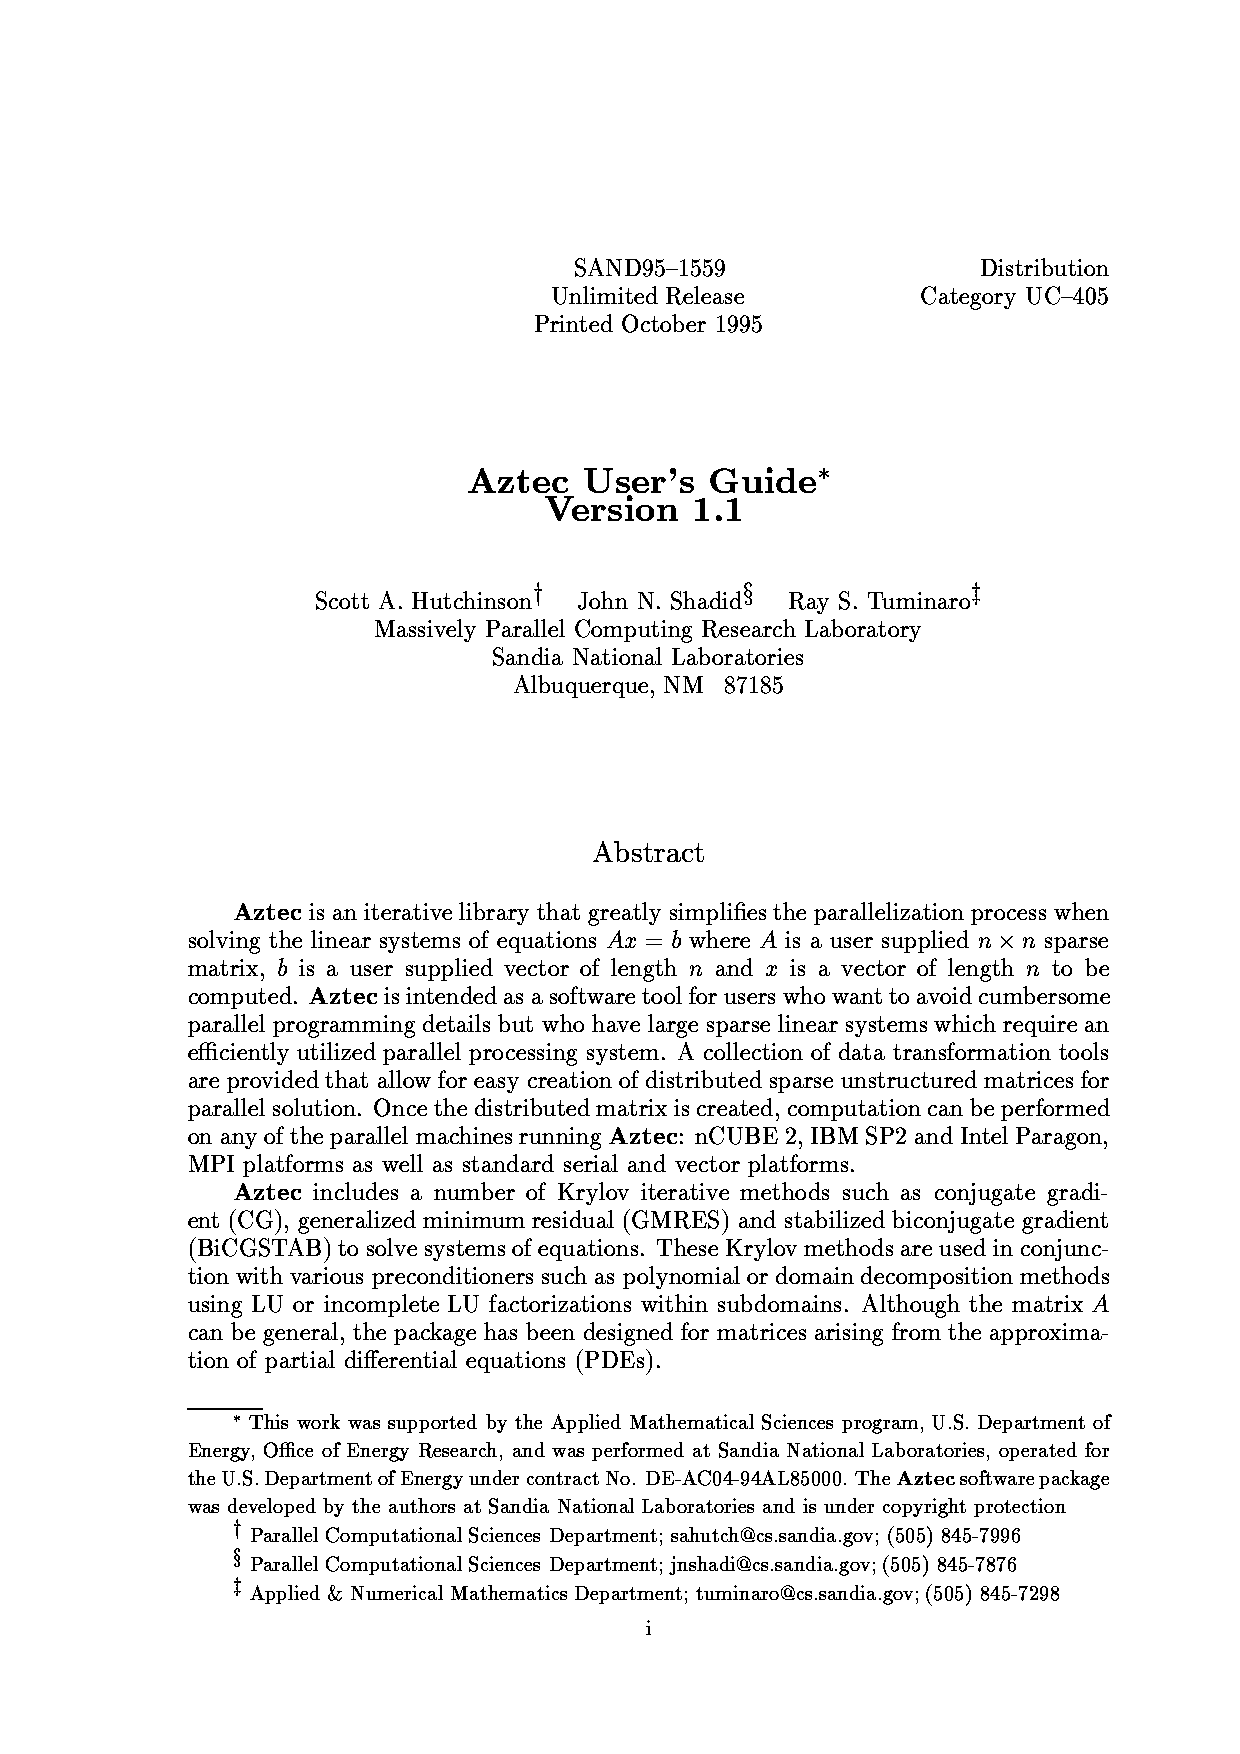
\includegraphics[width=11.0cm]{manual.jpg}
  \caption{Algorithm flowchart of PLaS coupled to a flow solver.}
  \label{fig:Flowchart}
\end{figure}

\subsection{General principle of PLaS}
\label{subsec:principle}

From figure \ref{fig:Flowchart} we see the general operational principle of PLaS coupled to a flow solver. PLaS updates the trajectories (velocity and position) of a set of dispersed entities at every time step of the flow solver. This is applied by using the Eulerian-Lagrangian approach, where Lagrangian equations of motion are solved for every particle, bubble or droplet to obtain its position and velocity. All dispersed entities are tracked sequentially, one after the other. The velocity field of the carrier phase serves as input for PLaS, since the continuous phase velocity is the driving mechanism for the motion of the dispersed entities. Moreover, PLaS computes back-coupling terms, which can be plugged into the equations of the flow solver (Navier-Stokes or Euler) in the form of mass and momentum sources. This is done in order to allow the flow solver to take into account the presence of the dispersed phase.

\subsection{Interfacing PLaS with a flow solver}
\label{subsec:interf}

The data interface between PLaS and the flow solver is bilateral. To call PLaS from the flow solver, three interface functions are accessible from outside the code:

\begin{itemize}
\item The initialization routine {\tt{initPLaS()}} allocates the memory needed by PLaS and has to be called before solving the flow (i.e. before the time loop).
\item The main routine {\tt{runPLaS()}} is the core of the whole program. A detailed description of its functionality is given in section \ref{subsec:mainroutine} of this manual. The main routine should be called from the flow solver after updating the velocoty field (i.e. after a system solve ans a solution update, but before starting the next time step).
\item The termination routine {\tt{terminatePLaS()}} de-allocates memory and finalizes PLaS.
\end{itemize}

These functions are declared in {\tt{/include/plasinterface.h}} and implemented in {\tt{/src/plas.c}}.

On the other hand, a couple of functions to provide data to PLaS have to be implemented in the flow solver chosen to couple PLaS to. These functions are declared as well in {\tt{/include/plasinterface.h}}. If these functions are not implemented in the flow solver, it will not be possible to link to the PLaS library. This leads to the fact that interfacing PLaS to any flow solver implies some initial programming work. At the present state, PLaS is coupled to the 2D/3D incomressible Finite Element Navier-Stokes solver Morpheus as well as to the 2D/3D Finite Volume Navier-Stoeks solver of the COOLFluiD framework. In these flow solvers, the interafce to PLaS alrerady exists.

In order to link PLaS to a flow solver, one has to include the PLaS interaface header file in the makefile of the flow solver by adding he follwing line:

{\tt{'CFLAGS += -I/\$(PLAS)/plas/include/plasinterface.h'}}

Here, {\tt{\$(PLAS)}} is the working directory you installed PLaS to. To link to the PLaS library archive to the flow solver, the following line has to be added:

{\tt{'LIBS += /\$(PLAS)/plas/lib/plas.a'}}

As described above, the header file {\tt{/include/plasinterface.h}} contains all necessary information to interface PLaS with a flow solver. Its features are structured as follows:

\begin{itemize}
\item Declaration of all data structures used by PLaS.
\item Declaration of the PLaS interface functions accessible from outside. These fuctions are implemented in {\tt{/src/plas.c}}.
\item Declaration of all interface functions to be implemented on the flow solver side.
\end{itemize}

\newpage
\section{The structure of PLaS}
\label{sec:structure}

In the following, an overview of the code structure of PLaS is given. The whole code is written in standard C language. A main principle of programming PLaS is to produce well-structured and readable code, making it as easy as possible for new users and developers to get into the program. All functionality is implemented in a modular way, where files and subroutines are grouped by functional aspects. Another important requirement in this scope is that file, function and variable names shoulod be self-explanatory.

\subsection{PLaS file and function structure}
\label{subsec:filefunc}

The functionality of the PLaS library is structured in various files and functions. The main routines {\tt{initPLaS()}}, {\tt{runPLaS()}} and {\tt{terminatePLaS()}}, which are accessible from outside, are located in {\tt{/src/plas.c}}, as described in section \ref{subsec:interf}.

All other functions of PLaS are internal routines and are not accessible from outside. All internal routines are declared in {\tt{/include/plas.h}} and implemented in the different files in the {\tt{/src}} directory. Their functionality will be described in section \ref{sec:routines}

\subsection{PLaS data structure}
\label{subsec:datastruct}

The data structure of PLaS is encapsulated in various {\tt{struct}} data types. All data structure declaration is included in {\tt{/include/plasinterface.h}}, making it accessible from outside PLaS. To instantiate all necessary PLaS data, a single instance of the data type {\tt{PLAS\_DATA}} has to be created in the flow solver. This instance has to be passed to the PLaS interface functions by pointer. In this way, it is assured that all PLaS data has got program lifetime of the flow solver.

The structure {\tt{PLAS\_DATA}} consists of the follwing sub-structures:

\begin{itemize}
\item {\tt{PLAS\_ENTITY\_DATA}} contains all information about a single dispersed entity (position, velocity, diameter...).
\item {\tt{PLAS\_PHASE\_DATA}} contains all information about dispersed phase quantities on the mesh points of the flow solver (number density, volume fraction, average dispersed phase velocity and diameter...).
\item {\tt{PLAS\_STATS}} contains counters and averaged characteristic quantities of the dispersed phase for the statistics output.
\item {\tt{PLAS\_INPUT\_PARAM}} contains all data provided by the PLaS input file {\tt{PLaS.param}}.
\item {\tt{PLAS\_RUNTIME\_PARAM}} contains data given to PLaS by the flow solver (flow and mesh dimensions, flow properties...).
\end{itemize}

\subsection{The PLaS input file}
\label{subsec:inpfile}

The PLaS code expects the presence of a data input file called {\tt{PLaS.param}} in the directory from where you execute the flow solver. Without this data file, PLaS will not be able to run. An example {\tt{PLaS.param}} file is provided in {\tt{/tools}}. The following parameters have to be specified in the PLaS input file:

\begin{itemize}
\item {\bf Maximum number of entities}: To avoid re-allocation memory, a maximum number of dispersed entities is required, which cannot be exceeded during runtime. The user should carefully set this parameter to get a good balance between allocated memory and the actual number of particles, bubbles or droplets in the simulation.
\item {\bf Restart from initial distribution}: Set to '0' in case of no restart, set to '1' for loading a {\tt{PLaS\_Positions.sol}} file from a previous calculation.
\item {\bf Number of initially distributed entities}: Number of randomly placed entities at the first iteration. Set to '0' for no entities. The initial velocities are interpolated form the fluid velocity at the entitiy position.
\item {\bf Diameter of dispersed entities}: Three parameters have to specified in this line:
\begin{itemize}
\item {\bf Diameter distribution type}: Set to '0' for constant diameter, set to '1' for normal distribution, set to '2' for log-normal distribution.
\item {\bf Diameter}: Value for the (mean) diameter $d$.
\item {\bf Standard deviation}: In case of constant diameter, this parameter has no effect, but still it has to be included to avoid a failiure in reading the file, for a normal distribution it is the standard deviation $\sigma>0$ and for a log-normal distribution the geometric standard deviation $\sigma_g=e^\sigma>1$.
\end{itemize}
\item {\bf Density of dispersed phase}: Value for the dispersed phase density $\rho_d$
\item {\bf Flow type}: Set to '0' for particulate or droplet flow, set to '1' for bubbly flow.
\item {\bf Momentum back-coupling}: Set to '0' for no mometum back-coupling through source terms in the fluid momentum equation, set to '1' to include it.
\item {\bf Volume fraction back-coupling}: Set to '0' for no volume fraction back-coupling  through source terms in the fluid continuity equation, set to '1' to include it.
\item {\bf Collision model}: Set to '0' for no collision model, set to '1' for uncorrelated Sommerfeld's collision model, set to '2' for correlated Sommerfeld's collision model.
\item {\bf Slip-shear lift force}: Set to '0' to exclude it, set to '1' to include it. Does only have an effect for bubbly flow.
\item {\bf Coupling force distribution method}:Set to '1' for the Particle-in-cell method (distribution only to the nearest node), set to '2' for distribution over the surrounding nodes.
\item {\bf Production domains}: In the first line, enter the number of production domains for dispersed entities. This number sets the number of following lines, each of them for one separated production domain. A production domain has to be specified by a number of parameters:
\begin{itemize}
\item The first number specifies the geometric shape of the production domain. Set '0' for none, set '1' for a line, set '2' for a rectangle or brick, set '3' for a circle, sphere or ellipsoid. This number is followed by a set of 6 parameters to specify the location and size of the production domain.
\item In case of a line the 6 parameters are the coordinates of the starting and ending points ($x$,$y$,$z$) of the line.
\item In case of a rectangle or brick, the 6 parameters are the coordinates of two diagonal nodes of the brick ($x$,$y$,$z$). Set a pair of coordinates equal to have a rectangle.
\item In case of a circle, sphere or ellipsoid, the first 3 parameters are the coordinates of the middle point, while the last 3 parameters are the radii ($x$,$y$,$z$). Set the radii equal to have a circle or sphere. 
\item In case of 2D, the $z$-coordinates have no effect in all the upper cases, but still they have to be included to avoid a failiure in reading the file.
\end{itemize}
\item {\bf Production factor}: Specifies how many entities per second are generated in each production domains.
\item {\bf Periodic boundaries}: If set to '0', entities will exit through periodic bloundaries of the flow, if set to '1', entities will be transported through them together with the flow.
\end{itemize}

\newpage
\section{Functionality of the PLaS routines}
\label{sec:routines}

As mentioned above, the functionality of PLaS is encapsulated in files and subroutines by functional aspects. Besides the main file {\tt{/src/plas.c}} described in section \ref{subsec:interf}, the folder {\tt{/src}} contains the following files:

\begin{itemize}
\item {\tt{plas\_auxiliary.c}}: Small auxiliary routines like a sorting routine and a random number generator.
\item {\tt{plas\_boundary.c}}: Functionality related to boundaries like the determination of particles leaving the domain, the wall distance calculation and the wall bouncing model.
\item {\tt{plas\_celldata.c}}: Calculation of cellwise data contained in the data structure {\tt{PLAS\_PHASE\_DATA}}.
\item {\tt{plas\_collisions.c}}: Includes the collision and coalescense models.
\item {\tt{plas\_coupling.c}}: Calculation of the back-coupling momentum and volume fraction terms to be passed to the flow solver.
\item {\tt{plas\_create.c}}: Initial entity distribution and entity generation in the production domains.
\item {\tt{plas\_flow.c}}: Calculation of flow properties like the fluid velocity at the entity position, the vorticity, the darg and lift coefficients and the dispersed phase Reynolds number.
\item {\tt{plas\_geometry.c}}: Contains all geometrical calculations that interface the computational mesh of the flow solver as well as all matrix and vector calculations.
\item {\tt{plas\_mpi.c}}: Contains interfaces to the MPI routines used.
\item {\tt{plas\_pass.c}}: In case of a parallel computation, the passing of dispersed phase information between the processes is implemented here.
\item {\tt{plas\_read.c}}: Reading and broadcasting of input parameters.
\item {\tt{plas\_search.c}}: Search routines to locate dispersed entities in the computationsl mesh of the flow solver.
\item {\tt{plas\_trajectory.c}}: Calculation of the entity trajectory (velocity and position).
\item {\tt{plas\_write.c}}: Writing out solution and statistics.
\end{itemize}

All functions contained in the above files are declared in a single header file {\tt{/include/plas.h}}, which provides a very good functional overview of the code.

\subsection{Main routines}
\label{subsec:mainroutine}

The three main rotines in {\tt{/src/plas.c}} were already discussed in section \ref{subsec:interf}. They are as follows:

\begin{itemize}
\item {\tt{void initPLaS(PLAS\_DATA*)}};
\item {\tt{void runPLaS(PLAS\_DATA*)}};
\item {\tt{void terminatePLaS(PLAS\_DATA*)}};
\end{itemize}

Each of the main routines receives a pointer to the instance of the main data structure {\tt{PLAS\_DATA}} as described in section \ref{subsec:datastruct}. The initialization and termination routines must only be called once at the start and end of the flow solver respectively. All PLaS relevant data allocation and de-allocation is performed there. The routine {\tt{runPLaS()}}, however, is called at every time the dispersed phase trajectories have to be updated, i.e. at every time step of the flow solver after updating the flow field.

When PLaS has to access data from the flow solver, this happens through the call-back routines declared in {\tt{/include/plasinterface.h}}. Those routines have to be implemented in the flow solver, as stated in section \ref{subsec:interf} and provide the following data:

\begin{itemize}
\item Information about the grid topology (nodes, elements and connectivity)
\item Information about the boundaries of the computational domain.
\item The velocity field of the carrier phase at time steps $n$ and $n-1$.
\end{itemize}

PLaS is a procedural C code, therefore the main routine {\tt{runPLaS()}} is called and run through from top to bottom at every time step of the flow solver. In the following, its functionality is described step by step:

\begin{itemize}
\item Read the input parameters from the {\tt{PLaS.param}} data file.
\item Broadcast the input parameters in case of a parallel computation.
\item Initialize counters and statistical data.
\item Impose an initial distribution of dispersed entities (random or from file) to the flow field in case of the first call of {\tt{runPLaS()}}.
\item Impose boudary conditions for the dispersed phase (i.e. create new entities at defined production domains).
\item Loop over all dispersed entities and sequentially update their trajectories
\begin{itemize}
\item According to a stability criterion (Lagrangian time step), perform the trajectory updates in sub-steps.
\item Compute fluid velocity at entity position and its derivatives in space and time.
\item Compute fluid vorticity.
\item Compute relative velocity, flow coefficients, entity Reynolds number and response time.
\item Update the trajectory (velocity and position).
\item Include wall bounces
\item Check if entities are leaving the domain through peridoci boundaries ot outlets.
\item Check if entities have to be passed from one process to another in case of a parallel computation.
\item Include entity collisions and coalescense in case of bubbly flow.
\end{itemize}
\item Pass entity information between processes in case of a parallel computation.
\item Compute cellwise dispersed phase data (volume fraction, number density...).
\item Calulate the momentum and volume fraction back-coupling terms.
\item Compute and write statistics and trajectory information to data files.
\item Return back to the flow solver.
\end{itemize}

\end{document} 
